\documentclass[a0paper,portrait]{baposter}

\usepackage{lmodern}

\usepackage[utf8]{inputenc}
\usepackage[T1]{fontenc}
\usepackage{colortbl}
\usepackage{arydshln}
\usepackage{booktabs}
\usepackage{forest}
\usepackage{tcolorbox}
\usepackage{multicol}
\usepackage{multirow}

\newcommand{\compresslist}{
\setlength{\itemsep}{0pt}
\setlength{\parskip}{1pt}
\setlength{\parsep}{0pt}
}

\newenvironment{boenumerate}
{\begin{enumerate}\renewcommand\labelenumi{\textbf\theenumi.}}
{\end{enumerate}}

\definecolor{mygray}{RGB}{226, 226, 226}
\definecolor{myred}{RGB}{252, 142, 142}
\definecolor{mygreen}{RGB}{147, 255, 143}
\definecolor{myblue}{RGB}{144, 155, 255}
\definecolor{myyellow}{RGB}{253, 253, 143}
\definecolor{mypurple}{RGB}{255, 142, 250}

\definecolor{bordercolor}{RGB}{223,165,56}
\definecolor{backgroundcolor}{RGB}{41,134,204}

\begin{document}
\begin{poster}
{
grid=false,
headerborder=open, % Adds a border around the header of content boxes
colspacing=1em, % Column spacing
bgColorOne=white, % Background color for the gradient on the left side of the poster
bgColorTwo=white, % Background color for the gradient on the right side of the poster
borderColor=bordercolor, % Border color
headerColorOne=backgroundcolor, % Background color for the header in the content boxes (left side)
headerColorTwo=backgroundcolor, % Background color for the header in the content boxes (right side)
headerFontColor=white, % Text color for the header text in the content boxes
boxColorOne=white, % Background color of the content boxes
textborder=rounded, %rectangle, % Format of the border around content boxes, can be: none, bars, coils, triangles, rectangle, rounded, roundedsmall, roundedright or faded
eyecatcher=false, % Set to false for ignoring the left logo in the title and move the title left
headerheight=0.11\textheight, % Height of the header
headershape=rounded, % Specify the rounded corner in the content box headers, can be: rectangle, small-rounded, roundedright, roundedleft or rounded
headershade=plain,
headerfont=\Large\textsf, % Large, bold and sans serif font in the headers of content boxes
%textfont={\setlength{\parindent}{1.5em}}, % Uncomment for paragraph indentation
linewidth=2pt % Width of the border lines around content boxes
}

%
%-----------------------------
%	TITLE AND AUTHOR NAME
%-----------------------------
%
{
\vspace{0.5em}
\textsf{Unveiling the Parallel Function Hypothesis on Personal Pronouns: A Corpus Analysis Utilizing Eye-Tracking Data}
}
{
\sf\vspace{-0.1em} \\
\textbf{Yue Chen}\\
\small{\texttt{yuechen218@ucla.edu} \quad \textbf{Department of Linguistics, The University of California, Los Angeles}}
}
{
\includegraphics[width=4cm,keepaspectratio]{figures/SealUCLA.PNG}}


\headerbox{1. Introduction}{name=introduction,span=1,column=0,row=0}{

This study investigates the influence of the \textbf{\color{blue}Parallel Functioning Hypothesis} on first fixation duration, number of fixations, and number of skips during sentence processing by using the \textbf{\color{blue}LARC-ID} eye-tracking dataset.
}


\headerbox{2. Background}{name=background,span=2,column=1}{

\textbf{Parallel Functioning Hypothesis (PFH)}
\\
Pronoun interpretation is influenced by both linguistic contexts, such as syntactic structures, social cues, eye gaze, and physical gestures  \cite{arnold2015effects} \cite{chien1990children}.
In complex sentences, the presence of the pronoun and its referential noun phrases \textbf{(NPs)} within the same grammatical functional category leads to Parallel Function Pronoun Resolution 
\textbf{(PFR)}\cite{sheldon1974role}\cite{grober1978parallel}. PFR results in easier and quicker processing when the pronouns and their referents fall into the same grammatical function category (Parallel Function), compared to Non-Parallel Function Pronoun Resolution \textbf{(NPFR)}
}

\headerbox{3. Research Question}{name=prompt,span=1,column=0,below=introduction}{

\begin{itemize}
    \item From a naturalistic reading perspective will the personal pronoun regulation obey the Parallel Functioning Hypothesis?
    \item Will the different grammatical functions of personal pronouns (SS, SO, OS) influence how people process referents?
    \item Will different sentence structures (inter and intar) influence how people process referents?
    \item How do previous knowledge and experiences influence an individual's pronoun resolution?

\end{itemize}

}

\headerbox{4. Data Set}{name=model,span=1,column=0,below=prompt}{
\small
We evaluate the following corpus:
\begin{itemize}
    \item The \textbf{\color{blue}LARC-ID} eye-tracking dataset \cite{harris2021angeles} 
    \item 15 college students (10 females, 5 males) were recruited
    \item All participants were native English speakers with a mean age of 19 years (SD = 1.13 years), ranging from 18 to 22 years
    \item All participants had some college experience, with an average of 2 years (range: 1-4 years)
\end{itemize}

}

\headerbox{5. Data Annotation}{name=conclusion,span=1,column=0,below=model}{
\small
\textbf{12} sentences were selected
         \begin{itemize}
         \item 6 PF sentence and 6 NPF sentences
         \end{itemize}
Four main areas of a sentence
     \begin{itemize}
        \item Target \textbf{\color{blue}subject} (the referent of the pronoun)
       \item  Target \textbf{\color{blue}pronoun}
       \item  Pronoun Region A (two words \textbf{\color{blue}before} the target pronoun)
       \item  Pronoun Region B (two words \textbf{\color{blue}after} the target pronoun)
      \end{itemize}

}

\headerbox{6. Result: Comparison Between PF and NPF Sentences}
{name=Result1,column=1,span=2,below=background}{
 {
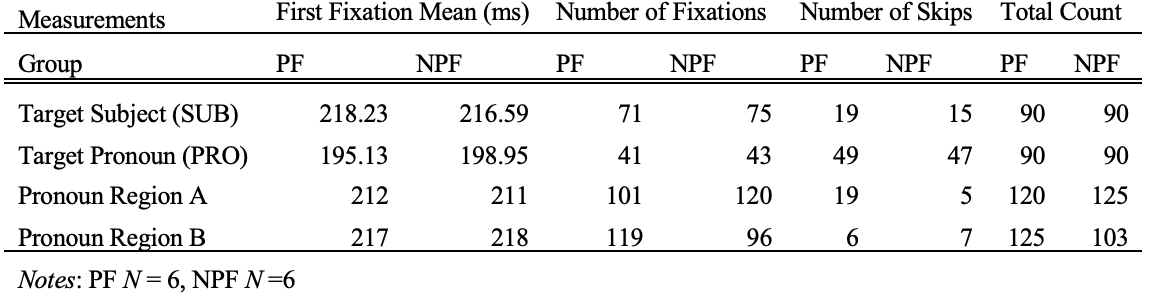
\includegraphics[width=15cm,keepaspectratio]{figures/first_fixation.png}}
 }
 
\headerbox{7. Result: Comparison Between SO SS and OS}
{name=Result2,column=1,span=2,below=Result1}{
 {
 \textbf{Comparison Between PF and NPF Sentences}
 \\
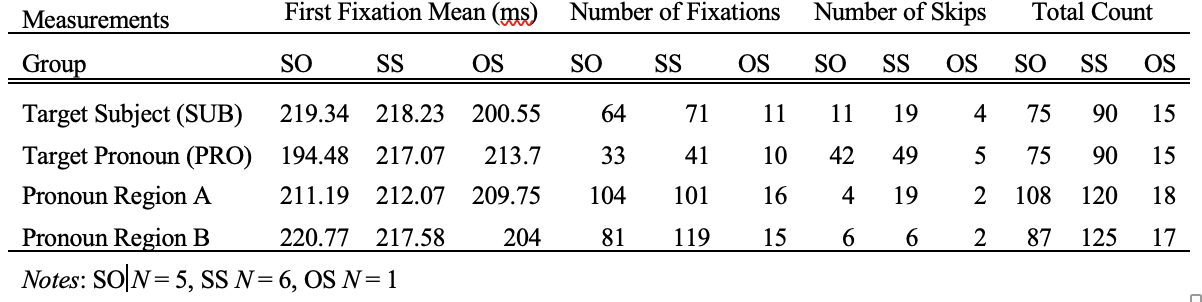
\includegraphics[width=15cm,keepaspectratio]{figures/SO_SS_OD.png}}
 }
 
\headerbox{8. Result: Comparison Between Intar and Inter sentences}
{name=Result3,column=1,span=2,below=Result2}{
 {
 \textbf{Comparison Between PF and NPF Sentences}
 \\
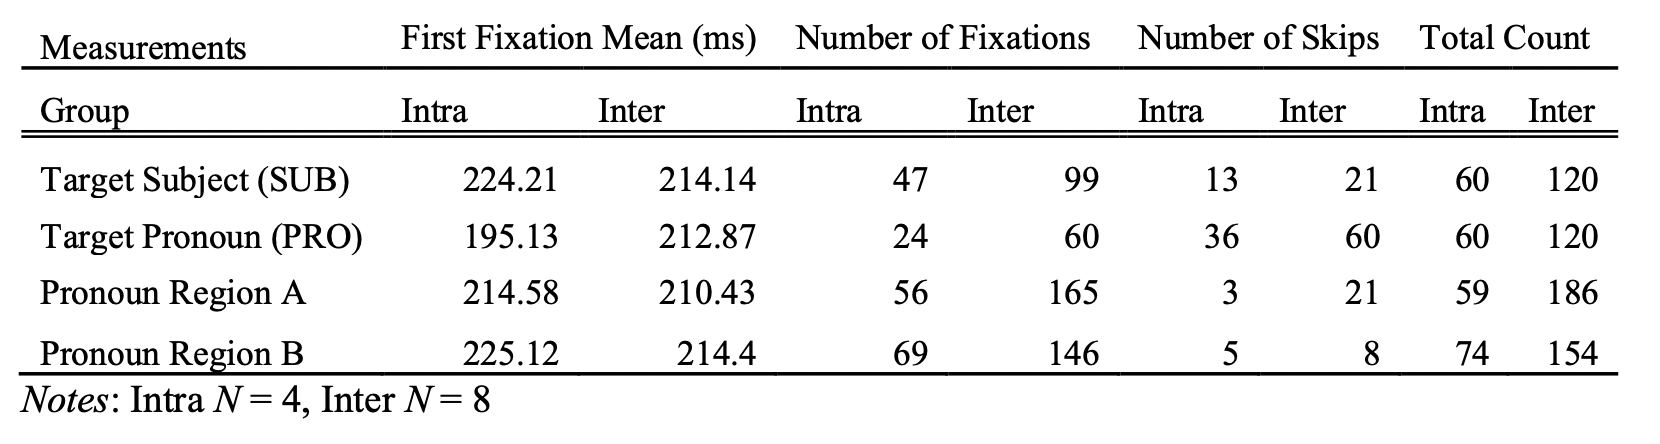
\includegraphics[width=15cm,keepaspectratio]{figures/Inter_Intra.png}}
 }

\headerbox{9. Conclusion}{name=r4,span=2,column=1,below=Result3}{
\begin{itemize}
    \item There are \textbf{\color{blue}minimal differences} between PF and NPF sentences, failing to provide positive support in favor of this hypothesis. 
    \item The intrasentential structures lead to \textbf{\color{blue}longer} first fixation duration for the target subject, target pronoun, and both pronoun regions compared to intersentential structures. 
    \item The grammatical positions of the subjects and the pronouns indicate that when the subject and pronoun are in the \textbf{\color{blue}subject-object position}, participants exhibit \textbf{\color{blue}longer first fixation duration} at the subject and \textbf{\color{blue}shorter first fixation duration} at the target pronoun.
    \end{itemize}
}

\headerbox{10. Acknowledgement}{name=acknowledgement,span=2,column=1,below=r4,above=bottom}{
I am deeply grateful to my undergraduate thesis supervisor Dr. Jesse Harris from UCLA for his guidance and help throughout this project; Dr. Stephanie Rich for her help with data collection; the UCLA linguistics department for providing financial support for this project; all members of the UCLA language processing lab for their comments and suggestions and the participants who participated in this study.

}


\headerbox{11. References}{name=references,column=0,span=1,below=conclusion,above=bottom}{
\scriptsize
% \small % Reduce the font size in this block
\renewcommand{\section}[2]{\vskip 0.05em} % Get rid of the default "References" section title
% \nocite{*} % Insert publications even if they are not cited in the poster
\bibliographystyle{apalike}
\bibliography{poster}

}

\end{poster}
\end{document}
